\documentclass[a4paper,12pt]{scrartcl} % From KOMA-script
\usepackage[margin=1in]{geometry}
\usepackage{xcolor}
\usepackage{graphicx}
\usepackage{fancyhdr}
\usepackage{lipsum} % For filler text
\usepackage{amsthm}
\usepackage{times}
\usepackage{microtype}
\usepackage{listings}
\usepackage{amsmath, amssymb, amsfonts, amssymb, float, enumitem}
\definecolor{darkbg}{HTML}{1E1E1E}
\definecolor{darktext}{HTML}{E0E0E0}
\definecolor{theoremcolor}{HTML}{d3dce5}
\definecolor{answercolor}{HTML}{e9dfc0}
\definecolor{sectioncolor}{HTML}{dec3c3}
\pagecolor{darkbg}
\color{darktext}
\newenvironment{solution}
  {\par\color{answercolor}\textbf{Solution:}\ }
  {\par}
\newenvironment{prf}
  {\par\textbf{Proof:}\ }
  {\par}

\newcounter{customcounter}
\newcommand{\setcustomcounter}[1]{\setcounter{customcounter}{#1}}

\newtheoremstyle{darktheorem}
  {\topsep}{\topsep}
  {\itshape\color{theoremcolor}}{}
  {\bfseries\color{theoremcolor}}{.}{.5em}{}
\theoremstyle{darktheorem}
\newtheorem{theorem}{Theorem}[section]
\newtheorem{lemma}[theorem]{Lemma}
\newtheorem{proposition}[theorem]{Proposition}
\newtheorem{corollary}[theorem]{Corollary}
\newtheorem{definition}[theorem]{Definition}
\newtheorem{example}[theorem]{Example}
\newtheorem{exercise}[customcounter]{Exercise}

\usepackage{fancyhdr}
\pagestyle{fancy}
\setlist[enumerate]{label=(\alph*)}

% Clear default headers
\fancyhf{}
\renewcommand{\headrulewidth}{0pt}

% Set Author and Date in the top left
\fancyhead[L]{\textcolor{darktext}{\small Asher Christian \\ 006-150-286 \\ \today }}

\begin{document}


\title{\color{sectioncolor}HW 2 Math 151B}
\author{}
\date{}
\maketitle

% Apply fancyhdr on the title page
\thispagestyle{fancy}

\begin{exercise}
    Let $m$ be a positive integer and $x \ge 0$. Show that
    \[
        (1+x)^{m} \le e^{mx}
    .\] 
\end{exercise}
\begin{solution}
    we have
    \[
    e^{x} = 1 + x + \frac{x^2}{2!} + \frac{x^{3}}{3!} + ... 
    .\] 
    each term $\frac{x^{n}}{n!}$ is greater than or equal to $0$ since $x \ge 0$. thus
    \[
    e^{x} \ge 1 + x
    .\] 
    with equality holding only if $x = 0$.
    since powers preserve inequalities.
    \[
        e^{mx} = (e^{x})^{m} \ge (1+x)^{m}
    .\] 
\end{solution}

\begin{exercise}
    Suppose $\alpha > 0$ and $\beta > 0$. Let $\{s_n\}$ be a sequence that satisfies $s_0 = 0$ and 
    \[
        s_n \le (1+\alpha)s_{n-1} + \beta \hspace{1cm} n \ge 1
    .\] 
    \begin{enumerate}
        \item Show that $e_1 \le \beta$. Then use induction to show that
            \[
                s_n \le \beta[1 + (1+ \alpha) + (1+\alpha)^2 + ... + (1 + \alpha)^{n-1}], \hspace{1cm} n \ge 2
            .\] 
        \item sum the geometric series of the RHS of $(a)$ to show that
            \[
                s_n \le \frac{\beta}{\alpha}((1+\alpha)^{n}-1) \hspace{1cm} n\ge 2
            .\] 
        \item Combine $(b)$ with the result from Problem 1, show that
            \[
                s_n \le \frac{\beta}{\alpha}(e^{n \alpha} - 1), \hspace{1cm} n \ge 2
            .\] 
    \end{enumerate}
\end{exercise}
\begin{solution}
    \begin{enumerate}
        \item we have $s_1 \le (1 + \alpha) \cdot 0 + \beta \implies s_1 \le \beta$
            inductively if we have
            \[
            s_n \le \beta(1 + (1+\alpha) + (1 + \alpha)^2 + ... + (1+\alpha)^{n-1})
            .\] 
            implies that
            \[
                s_{n+1} \le (1+\alpha)s_n + \beta \le \beta(1+\alpha)(1 + (1+\alpha) + \dots + (1+\alpha)^{n-1}) + \beta
            .\] 
            \[
            = \beta((1+\alpha) + (1+\alpha)^2 + \dots + (1+\alpha)^{n}) + \beta = \beta(1 + (1+\alpha) + \dots + (1+\alpha)^{n})
            .\] 
            so $s_{n+1}$ satisfies the recurrence relation and $s_1$ satisfies the recurrence relation so it holds for all $n$.
        \item 
            we have
            \[
                a_{n-1} = 1 + (1+\alpha) + (1+\alpha)^2 + \dots + (1+\alpha)^{n-1}
            .\] 
            \[
                (1+\alpha)a_{n-1} = (1+\alpha) + (1+\alpha)^2 +  \dots + (1+\alpha)^{n}
            .\] 
            \[
                (1+\alpha-1)a_{n-1} = (1+\alpha)^{n} - 1
            .\] 
            \[
                a_{n-1} = \frac{(1+\alpha)^{n}-1}{\alpha}
            .\] 
            so we have
            \[
                s_n \le \beta a_{n-1} = \frac{\beta}{\alpha}((1+\alpha)^{n}-1)
            .\] 
        \item 
            we have
            \[
                (1+\alpha)^{n}-1 \le e^{\alpha n} - 1
            .\] 
            \[
            s_n \le \frac{\beta}{\alpha}((1+\alpha)^{n}-1) \le \frac{\beta}{\alpha}(e^{\alpha n} - 1)
            .\] 
    \end{enumerate}
    \begin{exercise}
        
    \end{exercise}
    \begin{solution}
        \[
        y''(t) = f_t + f f_y
        .\] 
        \[
        y'''(t) = \frac{d}{dt}f_t + \frac{d}{dt}(f f_y)
        .\] 
        \[
            \frac{d}{dt} f_t = f_{tt} + f_{ty} (\frac{dy}{dt}) = f_{tt} + f f_{ty}
        .\] 
        \[
        \frac{d}{dt}(f f_y) = (\frac{d}{dt}f) f_y + f (\frac{d}{dt} f_y)
        .\] 
        \[
            \frac{d}{dt}f_y = f_{yt} + f_{yy} \frac{d}{dt}y = f_{yt} + ff_{yy}
        .\] 
        \[
            \frac{d}{dt}(f f_y) = f_tf_y + f f_y^2 + ff_{ty} + f^2f_{yy}
        .\] 
        \[
            \frac{d}{dt}y''(t) = f_{tt} + ff_{ty} + f_tf_y + ff_y^2 + ff_{ty} + f^2f_{yy}
        .\] 
        \[
            = f_{tt} + 2ff_{ty} +  f^2f_{yy} + f_y(f_t + ff_y)
        .\] 
    \end{solution}
    \begin{exercise}
        
    \end{exercise}
    \begin{solution}
        \begin{enumerate}
            \item
            \[
           y(t) = \frac{1}{t}
           .\]  
           \[
           y' = -\frac{1}{t^2}
           .\] 
           \[
           -5ty^2 + \frac{5}{t} -\frac{1}{t^2} = \frac{-5t}{t^2} + \frac{5}{t} -\frac{1}{t^2} = -\frac{1}{t^2} = y'
           .\] 
           so $y(t) = \frac{1}{t}$ solves the IVP.
       \item 
           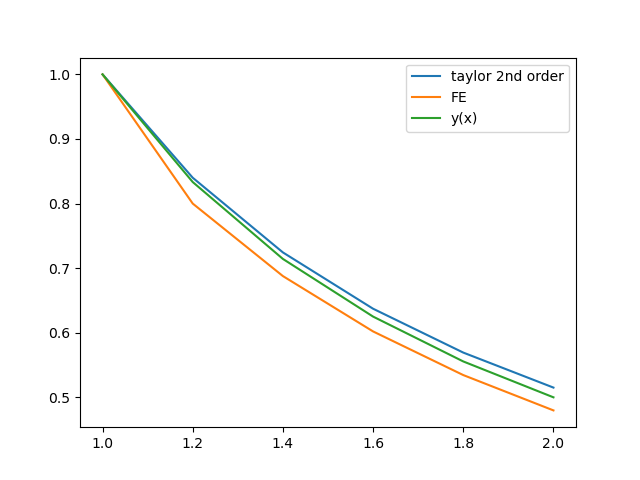
\includegraphics{output.png}
           \begin{lstlisting}
import matplotlib.pyplot as plt
def y(t):
    return t**(-1)
def f(t,y):
    return -5*t*(y**2) + 5/t - 1/(t**2)

def f_t(t,y):
    return -5*(y**2) - 5/(t**2) + 2/(t**3)

def f_y(t,y):
    return -10*t*y

def f_tt(t,y):
    return 10/(t**3) - 6/(t**4)

def f_ty(t,y):
    return -10*y

def taylor(y_n, t_n, h, f, f_t, f_y, f_tt, f_ty):
    return y_n + h*f(t_n,y_n) + (h**2)/(2) * (f_t(t_n,y_n) + f(t_n,y_n)*f_y(t_n,y_n))

def FE(y_n,t_n,h,f):
    return y_n + h*f(t_n,y_n)

x = np.arange(1,2.1,0.2)
output = y(x)
taylor_out = np.zeros_like(x)
fe_out = np.zeros_like(x)

taylor_out[0] = x[0]
fe_out[0] = x[0]
h = 0.2

for index, i in enumerate(x[:-1]):
    taylor_out[index+1] = taylor(taylor_out[index],i,h,f,f_t,f_y,f_tt,f_ty)
    fe_out[index+1] = FE(taylor_out[index],i,h,f)

print(taylor_out, fe_out, output, x)

plt.plot(x,taylor_out, label="taylor 2nd order")
plt.plot(x,fe_out, label = "FE")
plt.plot(x,output, label = "y(x)")
plt.legend()
plt.savefig("output.png")

           \end{lstlisting}
        \end{enumerate}
    \end{solution}
\end{solution}

\begin{exercise}
\end{exercise}
\begin{solution}
    $y' = f(t,y)$
    \[
        y(t_{n+1}) - y(t_n) = \int_{t_n}^{t_{n+1}}y'(t)dt
    .\] 
    Trapezoidal rule
    \[
    \int_{a}^{b}f(x)dx \approx \frac{(b-a)}{2}(f(a) + f(b))
    .\] 
    so
    \[
        y(t_{n+1}) - y(t_n) \approx \frac{h}{2}(f(t_n,y_n) + f(t_{n+1},y_{n+1}))
    .\] 
    to create the implicit trapezoidal method
    \[
        y_{n+1} = y_n + \frac{h}{2}(f(t_n,y_n) + f(t_{n+1},y_{n+1}))
    .\] 
    this is equivalent to
    \begin{align*}
        k_1 &= f(t_n+0h,y_n+h(0k_1 + 0k_2))\\
        k_2 &= f(t_n + h, y_n + \frac{h}{2}(k_1 + k_2))\\
        y_{n+1} &= y_n + h(\frac{k_1}{2} + \frac{k_2}{2})
    \end{align*}
    to create the butcher array
    \[
    \begin{array}{c|cc}
    0   & 0 & 0 \\
    1   & \frac{1}{2} & \frac{1}{2} \\
    \hline
        & \frac{1}{2} & \frac{1}{2}
    \end{array}
    \]
    \\
    If instead we use forward euler to find $y_{n+1}$ we get
    \[
        y_{n+1} = y_n + \frac{h}{2}(f(t_n,y_n) + f(t_{n+1}, y_n + hf(t_n,y_n)))
    .\] 
    This is equivalent to
    \begin{align*}
        k_1 &= f(t_n,y_n)\\
        k_2 &= f(t_n + h, y_n + hk_1)\\
        y_{n+1} &= y_n + \frac{h}{2}(k_1 + k_2)
    \end{align*}
    for a butcher array 
    \[
    \begin{array}{c|cc}
        0 & 0 & 0\\
        1 & 1 & 0\\
        \hline
          & \frac{1}{2} & \frac{1}{2}
    \end{array}
    .\] 
    \[
        k_2 = f(t_n + h, y_n + hk_1) = f + hf_t + hk_1f_y + \frac{1}{2}(f_{tt}(\xi,\eta)h^2 + 2f_{ty}(\xi,\eta)h^2k_1 + f_{yy}(\xi,\eta)h^2k_1^2)  
    \] 
    \[
        =f + h(f_t + ff_y) + h^2(\frac{f_{tt}(\xi,\eta)}{2} + ff_{ty}(\xi,\eta) + \frac{f^2f_{yy}(\xi,\eta)}{2})
    \] 
    now consider the local truncation error assuming $y_n = y(n)$
    \[
        \tau = y(t_{n+1}) - y_{n+1} = y(t_n + h) - y(t_n) - \frac{h}{2}(2f + h(f_t + ff_y) -h^2(\frac{f_{tt}(\xi,\eta}{2} + ff_{ty}(\xi,\eta) + \frac{f^2f_{yy}(\xi,\eta)}{2})
    .\] 
    but
    \[
    y(t_n + h) = y(t_n) + hy'(t_n) + \frac{h^2}{2}y''(t_n) + O(h^{3}) = y(t_n) + hf + \frac{h^2}{2}(f_t + ff_y) + O(h^{3})
    .\] 
    plugging in and grouping by $h$ terms we get
    \[
        \tau = y(t_n) - y(t_n) + h(f-f) + \frac{h^2}{2}(f_t+ff_y -f_t-ff_y) + O(h^{3}) -\frac{h^{3}}{4}(f_{tt}(\xi,\eta) + 2f f_{ty}(\xi,\eta) + f^2f_{yy}(\xi,\eta))
    .\] 
    \[
    = O(h^{3})
    .\] 

\end{solution}
\begin{exercise}
    
\end{exercise}
\begin{solution}
   \begin{enumerate}
       \item So far I feel like the connection between local truncation error and global error is important since we kind of just said that local truncation error
           being $O(h^{p+1})$ means that the system is $p$th order accurate, which implies that the global error is $O(h^{p})$ but formal justification of this would be great.
           I'm also curious how implicit methods are implemented in code. It was mentioned in class that other numerical methods are used to approximate the roots of the implicit functions
           but understanding how this might change the errors would be cool.
       \item So far this class is much better than my previous numerical methods course. I felt like the previous course placed too much emphasis on tedious calculations, but often those calculations are busy work, and I appreciate
           this course making the more tedious parts homework since they give a better understanding for the student and leave more time for the higher level discussions during class time. I really like the way the class is formatted.
   \end{enumerate} 
\end{solution}


\end{document}
